% Proposed solution: system architecture overview (issue #5).
% Fig. system.png comes from docs/architecture/ (#18); re-exporting it there
% updates the report.

\section{Proposed Solution}
\subsection{Architecture Overview}
The accelerator computes $C = AB$, where $A$ and $B$ are $N \times N$ matrices of signed $\mathrm{DATA\_W}$-bit operands and
\begin{equation}
C[i][j] = \sum_{k=0}^{K-1} A[i][k]\,B[k][j].
\label{eq:matmul}
\end{equation}
In Phase~1 the inner dimension $K$ equals $N$. Table~\ref{tab:params} lists the parameters. Every module takes them as Verilog parameters, so the array size and the data widths change in one place.

\begin{table}[t]
\centering
\caption{Design parameters}
\label{tab:params}
\footnotesize
\begin{tabular}{@{}llc@{}}
\toprule
Parameter & Meaning & Default \\
\midrule
$N$ & array size; $A$, $B$ and $C$ are $N \times N$ & 4 \\
$K$ & inner dimension (equal to $N$ in Phase~1) & 4 \\
$\mathrm{DATA\_W}$ & operand width, signed & 8 \\
$\mathrm{ACC\_W}$ & accumulator and result width, signed & 32 \\
$\mathrm{FRAC\_W}$ & fractional bits of the Q-format reading & 0 \\
$T$ & compute cycles, $K + 2N - 2$ & 10 \\
\bottomrule
\end{tabular}
\end{table}

\begin{figure*}[t]
\centering
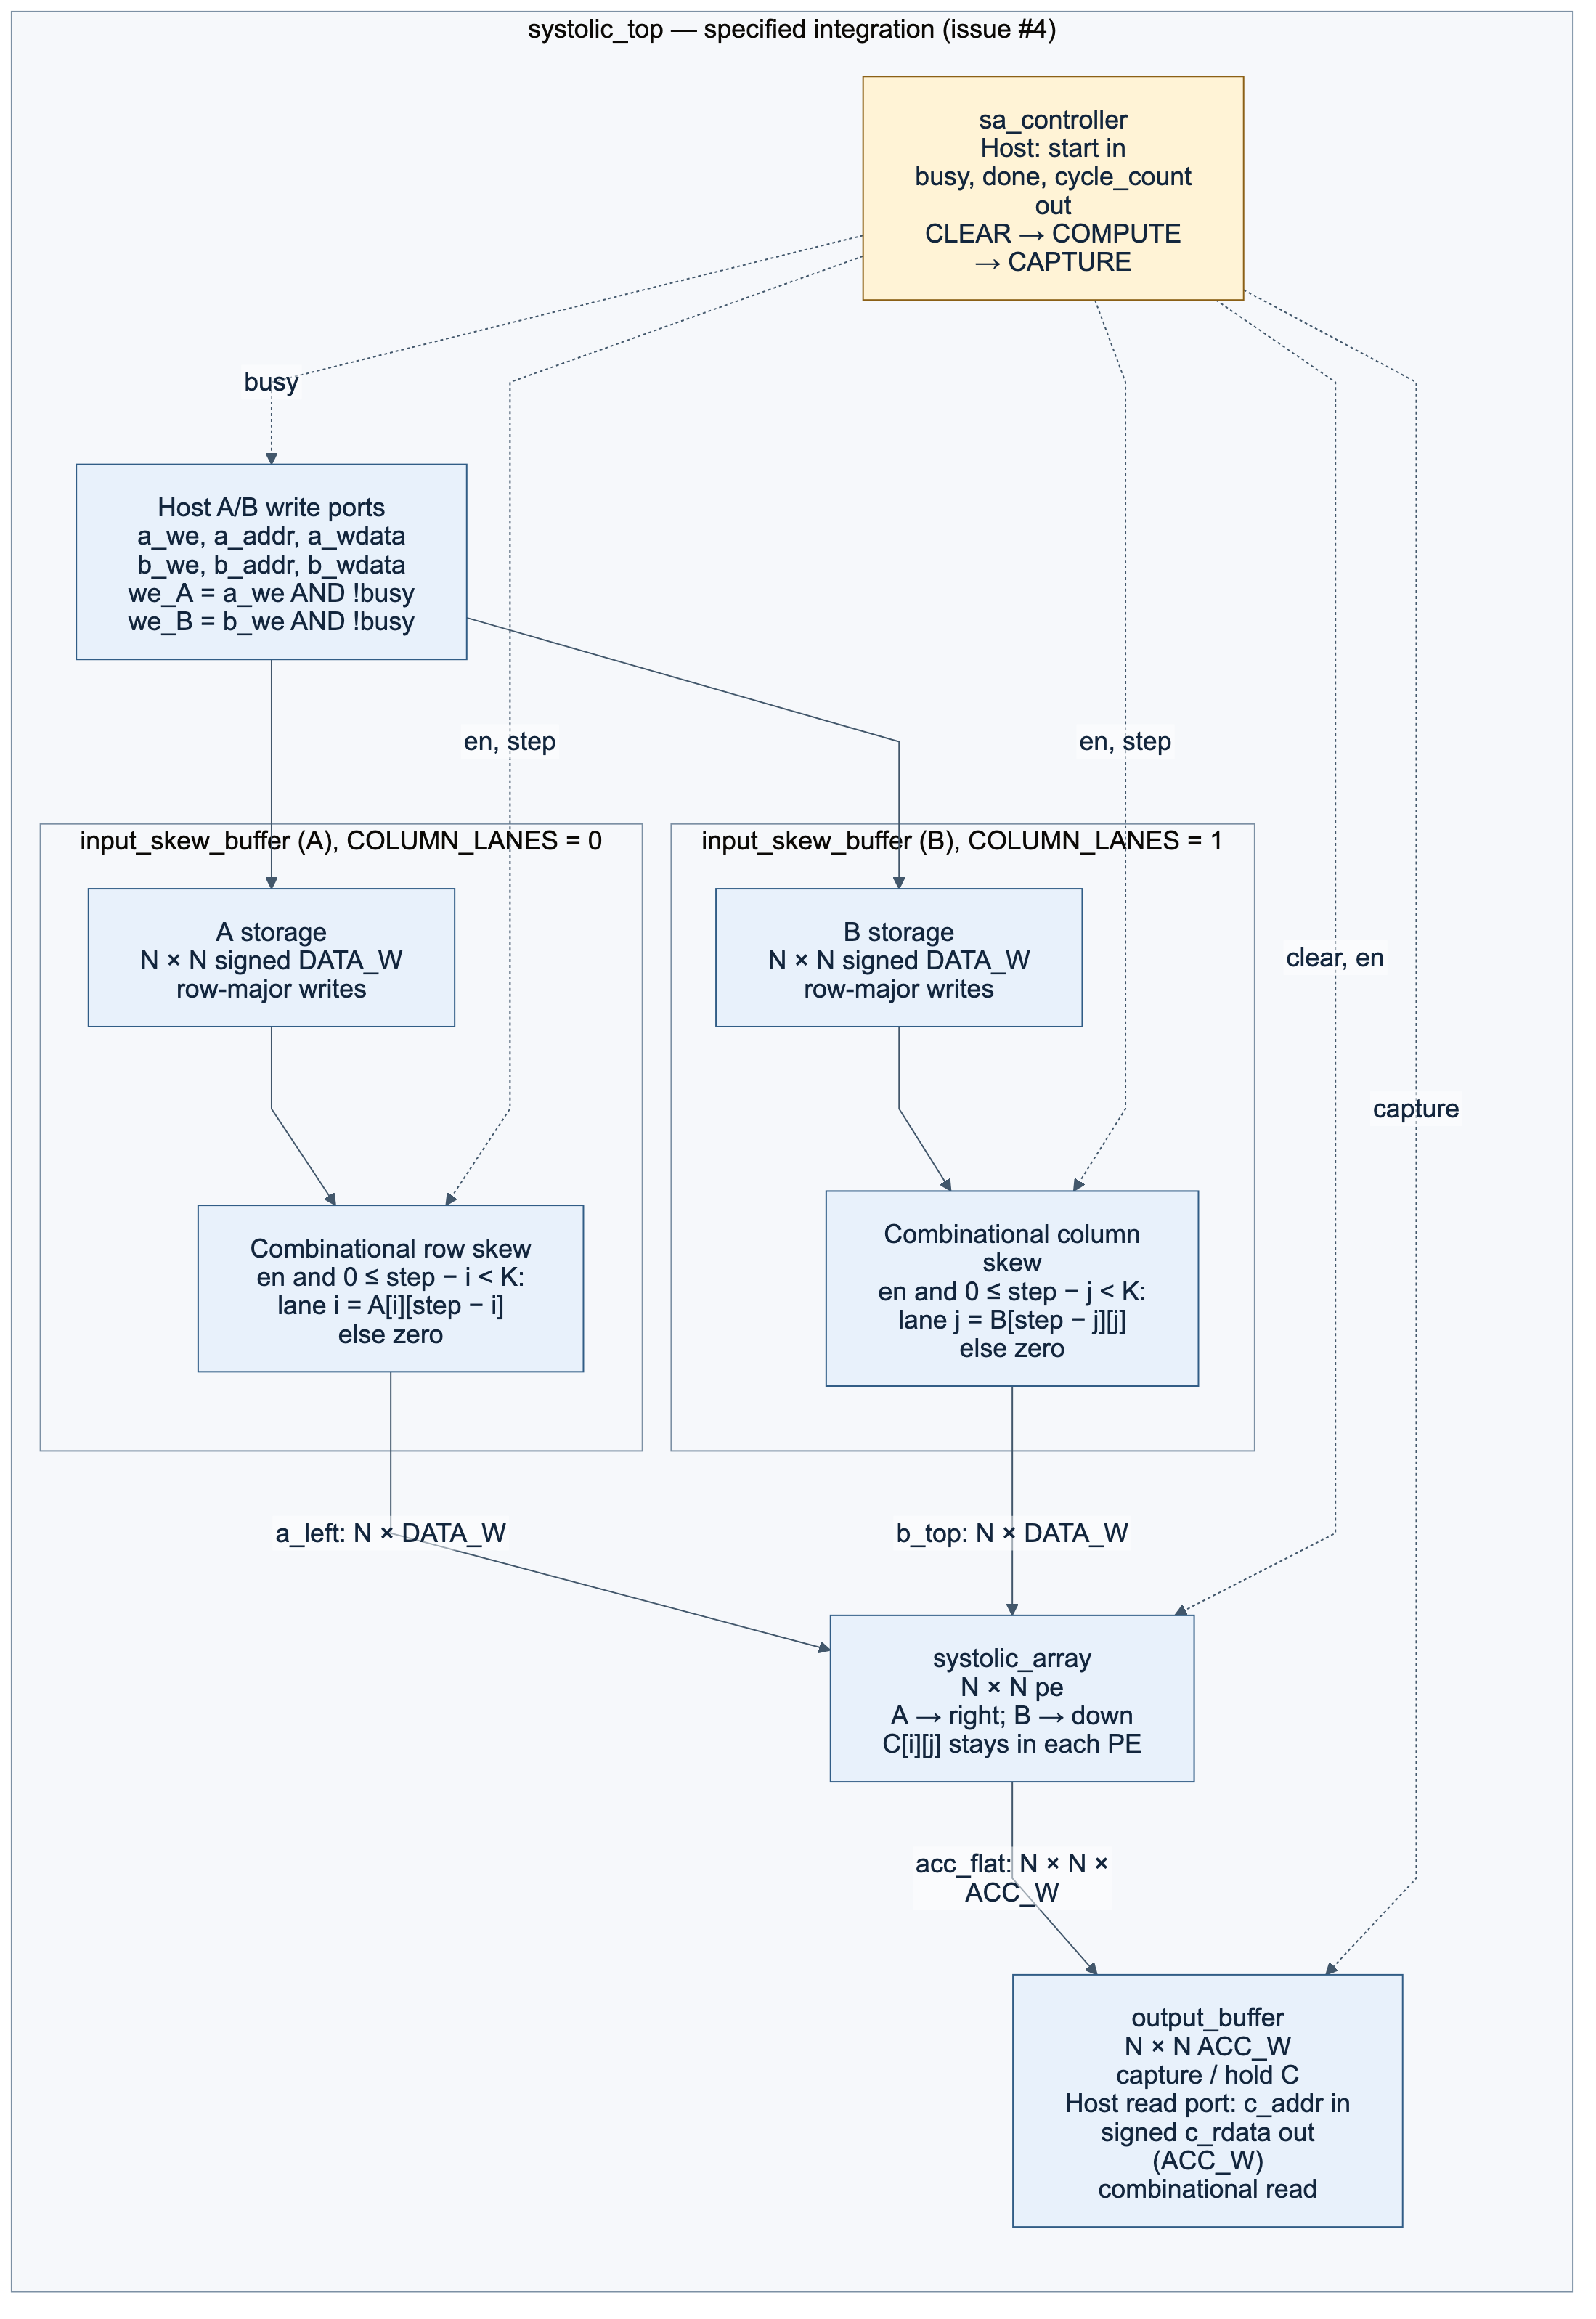
\includegraphics[width=\textwidth]{system.png}
\caption{System architecture. Solid arrows carry data and dashed arrows carry controller signals. Host writes reach the input skew buffers only while \texttt{busy} is low. Each buffer stores one matrix and selects its skewed lanes from \texttt{step}. The controller clears the array, enables it for $T$ steps and then captures the accumulators into the output buffer, which serves the read port.}
\label{fig:system}
\end{figure*}

The design has five blocks behind one host interface, shown in Fig.~\ref{fig:system}:
\begin{itemize}
\item \textbf{Two input skew buffers.} Each stores one operand matrix and feeds one edge of the array. The A buffer drives row $i$ of $A$ into the left edge $i$ cycles late. The B buffer drives column $j$ of $B$ into the top edge $j$ cycles late.
\item \textbf{The systolic array.} An $N \times N$ grid of PEs. PE $(i,j)$ multiplies the operands that reach it, adds the product to its accumulator, which holds $C[i][j]$, and passes $A$ to the right and $B$ down one cycle later. The PE is described in Section~III-B and the skew in Section~III-C.
\item \textbf{The output buffer.} Copies all $N^2$ accumulators in one cycle when a computation ends, and serves them to the host through a read port. The previous result therefore stays readable while the next product is computed.
\item \textbf{The controller.} A five-state machine that clears the array, runs the $T$ compute steps, and signals the capture and the end of the run (Section~III-D).
\end{itemize}

The host sees a small matrix data interface. It writes $A$ and $B$ one element at a time through two write ports with row-major addresses, pulses \texttt{start}, waits for \texttt{done}, and reads $C$ one element at a time through the read port. While \texttt{busy} is high, writes are ignored, so the operands of a running product cannot change. Between runs $A$ and $B$ keep their contents, so a host can replace one matrix and start again. A \texttt{cycle\_count} output reports how many cycles the last run took, which the testbenches use to check the latency.

A run proceeds as follows. On \texttt{start} the controller spends one cycle clearing every accumulator and forwarding register. It then runs $T = K + 2N - 2$ compute steps, during which the skewed operands cross the array and every PE adds its $K$ products. One more cycle copies the accumulators into the output buffer, and \texttt{done} rises. For $N = K = 4$, \texttt{busy} is high for $K + 2N = 12$ cycles.

The array performs $N^2 = 16$ MACs per cycle at its peak and computes the $N^2K = 64$ MACs of a $4 \times 4$ product in 10 compute cycles, against 64 cycles for a single sequential MAC unit: a speed-up of 6.4 on compute and 5.3 over all 12 busy cycles. Each PE is busy for $K$ of the $T$ cycles, so utilization is $K/T = 40\,\%$ at this size, because the wavefront needs $2N - 2$ cycles to fill and drain the array. Utilization approaches 100\,\% as $K$ grows. With one-element ports, loading $A$ and $B$ takes 16 cycles and reading $C$ another 16. A complete product including I/O therefore takes about 44 cycles, so at this size the narrow ports, not the array, limit throughput.

The arithmetic is exact integer arithmetic: the 32-bit accumulators cannot overflow at these sizes (Section~III-B), so the datapath needs no rounding or saturation. Operands can also be read as Q-format fixed-point numbers with $\mathrm{FRAC\_W}$ fractional bits, and each element of $C$ then has $2\,\mathrm{FRAC\_W}$ fractional bits. This changes only how the numbers are read, not the hardware.
